%!TEX root = ../../../adrien_gomar_phd.tex
\chapter{Introduction to aeroelasticity}
\label{cha:ael}

\chabstract{In this chapter, the basic elements
to understand aeroelasticity in turbomachinery and by extension
in contra-rotating open rotors are detailed. Firstly, the
definition and the basic equations governing dynamic
aeroelasticity are presented. The two main aeroelastic
phenomena that develop in turbomachinery,
namely forced response and flutter, are then presented.
The latter is investigated in this work and the computational
approach retained to simulate it, namely the \replaced{decoupled}{weak-coupling} approach,
is presented. The variables that are used to quantify the 
flutter boundary are finally presented.}


\newpage

\section{What is aeroelasticity}
\label{sec:what_is_ael}
%!TEX root = ../../../adrien_gomar_phd.tex

The study of aeroelasticity in turbomachineries takes its origin
in the first engines failure during the sixties~\cite{Dugundji2003}.
Also called dynamic aeroelasticity,
it is the interaction between three forces:
the aerodynamic ($\mathcal{A}$), the elastic ($\mathcal{E}$) and
the inertial forces ($\mathcal{I}$) as 
shown by the \citet{Collar1946} triangle represented in 
Figure~\ref{fig:ael_collar_triangle}. 
\begin{figure}[htp]
  \centering
  \includegraphics*[width=0.45\textwidth]{collar_triangle.pdf}
  \caption{Collar triangle for dynamic aeroelasticity.}
  \label{fig:ael_collar_triangle}
\end{figure}

From a structural point of view, 
the dynamic aeroelasticity is governed by
\begin{equation}
	M \ddot{x}(t) + D \dot{x}(t) + K x(t) = f(t)
	\label{eq:ael_motion_eq}
\end{equation}
where $M$, $D$ and $K$ are the structural mass, damping 
and stiffness matrices, respectively.
$x(t)$ and $f(t)$ denote the displacement 
and aerodynamic force vectors, respectively. The displacement
vector is defined relatively to the 
steady-state position of the system. In turbomachinery
and by extension in CROR, it is the steady-state position
in rotation.


\section{Main aeroelastic phenomena in turbomachinery}
\label{sec:ael_phenomena}
%!TEX root = ../../../adrien_gomar_phd.tex

\subsection{Forced response}
\label{sub:forced_response}

As shown previously in Sec.~\ref{sec:cror_unsteady}, wakes and
potentials effects give rise to unsteady fluctuations in 
CROR configurations. These fluctuations 
can generate large vibration levels on the blades.
When the structural modes are excited by the rotation speed
or its multiples, resonance can occur,
hence the term forced response. 
The frequency associated to the rotation speed or its multiples
is called Engine Order (EO).
At the design phase, one step to minimize forced response is
to use the Campbell diagram shown in Figure~\ref{fig:campbell}
which schematically represents such resonance.
Blue points show the crossing of engine order with 
the blade eigenfrequencies within the operating range. 
The Campbell diagram does not give any information about
the absolute level of vibration. Therefore, it is mostly
used to rank potential designs~\cite{Marshall1996}. This phenomenon
will not be studied in this thesis.
\begin{figure}[htp]
  \centering
  \includegraphics*[width=0.45\textwidth]{campbell.pdf}
  \caption{Campbell diagram with forced response (blue circles)
  and flutter behavior (red stars).}
  \label{fig:campbell}
\end{figure}


\subsection{Flutter}
\label{sub:flutter}

Flutter is defined as a self-excited, unstable 
self-sustained vibration. In turbomachinery, this is
more likely to appear on blades.
One of the most impressive
manifestation of flutter occurred on the Tacoma Narrows
bridge in November 7\textsuperscript{th}, 1940.
Four months after being built, the bridge experienced 
torsional flutter excited by a 
\mbox{$64$~km.h\textsuperscript{-1}} wind.
The first and second torsional modes were observed.
A few hours later, the bridge felt down as seen in 
Figure~\ref{fig:tacoma_bridge}. Hopefully, no human
was injured, but this event showed the importance
of taking into account the flutter phenomenon as
it is a very energetic event, that can lead to the failure of the system.
\begin{figure}[htp]
  \centering
  \subfigure[torsion mode]{
      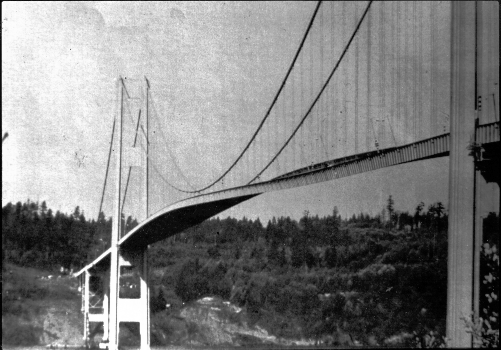
\includegraphics[height=.3\textwidth]{tac06.png}}
  \subfigure[failure of the bridge]{
      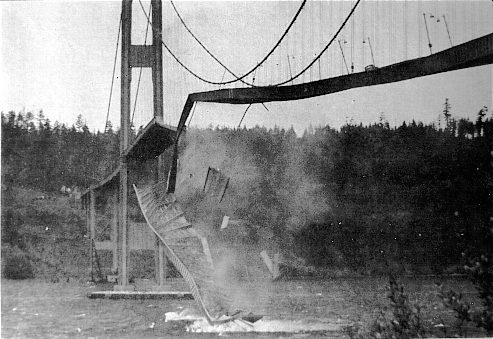
\includegraphics[height=.3\textwidth]{tac09.png}}
  \caption{Tacoma Narrows bridge flutter, from \citet{Smith1974}.}
  \label{fig:tacoma_bridge}
\end{figure}

Three vibration scenarios can appear, one leading to flutter.
The first scenario is the damped (or positively damped) 
vibration meaning
that the amplitude of the displacement decreases with respect to time, 
as shown in Figure~\ref{fig:flutter_damped}.
This is the most wanted behavior as the system tends to
a stable point. In this case, the blade is said to
be flutter-free for the studied mode.
The second scenario is the amplified (or negatively damped)
vibration, namely flutter, shown in Figure~\ref{fig:flutter_amplified}. 
This was the scenario that occurred on the Tacoma bridge. 
This scenario ultimately
leads to failure, which is not acceptable. This is particularly critical
on CROR configurations, as a blade failure might lead to 
the crash of the airplane as detailed in Sec.~\ref{sec:cror_challenges}.
The last scenario is the Limit Cycle Oscillation (LCO) vibration.
In this scenario, the deformation increases until a certain 
amplitude and then stays constant. This scenario is not
destructive by essence compared to the amplified scenario. However,
if the blade is repetitively excited by LCO, the blade
can fail because of structure fatigue.
\begin{figure}[htp]
  \centering
  \subfigure[damped (stable)]{
      \label{fig:flutter_damped}
      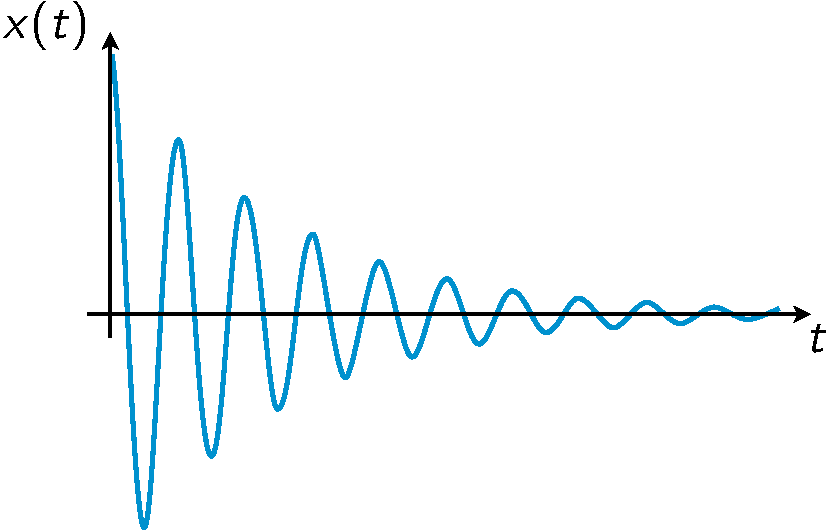
\includegraphics[width=.3\textwidth]{flutter_damped.pdf}}
  \subfigure[\replaced{linear flutter instability}{amplified (flutter)}]{
      \label{fig:flutter_amplified}
      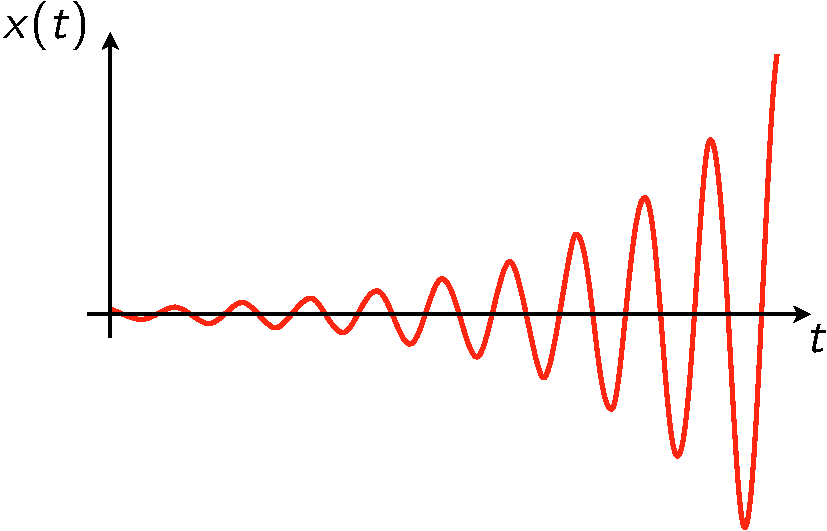
\includegraphics[width=.3\textwidth]{flutter_amplified.pdf}}
  \subfigure[limit cycle oscillation]{
      \label{fig:LCO}
      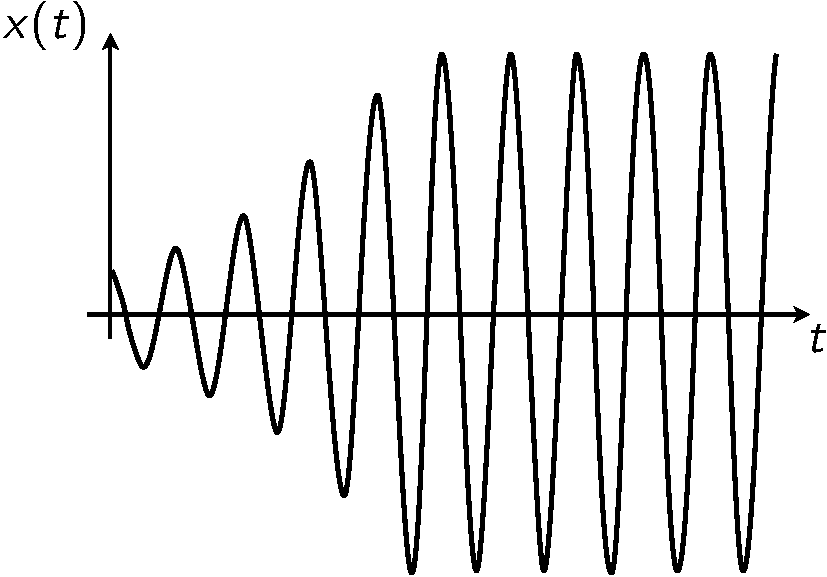
\includegraphics[width=.3\textwidth]{LCO.pdf}}
  \caption{Different vibration scenarios for the flutter phenomenon.}
\end{figure}

The development of one scenario over another one is linked to
the fluid response to the vibration of the blade. In fact,
if the aerodynamic loads projected on the direction of the displacement
is positive, this means that the vibration will be amplified. 
In opposite, if the force is in opposed direction, the vibration will be damped.
Therefore, the out-of-phase component of the aerodynamic force compared to
the displacement vector will give the sign of the aerodynamic damping.
The amplitude will give its strength. 

In this thesis, only the flutter boundary is assessed
and a \replaced{decoupled}{weak-coupling} approach is chosen
as detailed in the following Section.


\section{\texorpdfstring{\underline{C}}{C}omputational 
\texorpdfstring{\underline{A}}{A}ero\texorpdfstring{\underline{E}}{E}lasticity (CAE)}
\label{sec:cae}
%!TEX root = ../../../adrien_gomar_phd.tex

Solving Eq.~\eqref{eq:ael_motion_eq} analytically is generally 
not feasible. In fact, in turbomachinery, 
the flow exhibits non-linear features such as turbulence, shock and
boundary-layer interaction, to name but a few, that are out of reach for
analytical methods.

Two main strategies exist then for solving Eq.~\eqref{eq:ael_motion_eq}:
the strong-coupling and the \replaced{decoupled}{weak-coupling} strategies. The strong-coupling 
approach either solves the equation directly or two solvers are coupled to 
compute the aerodynamic and the structural response of the system.
The strong-coupling remains computationally expensive~\cite{Bartels2007}
and numerically stiff~\cite{Datta2008}. This approach
has been used to assess the
aeroelasticity of propellers~\cite{Ruiz-Calavera2012} and
CROR~\cite{Laban2010}. However, 
the strong-coupling remains 
computationally expensive~\cite{Bartels2007}.
It is therefore not used in this thesis.

Conversely, the \replaced{decoupled}{weak-coupling} approach has been widely used
in the turbomachinery aeroelasticity community~\cite{Marshall1996}.
This method uses a modal approach to identify the structural modes.
These modes are then prescribed with a harmonic motion in the aerodynamic
flow solver. The aerodynamic force is finally post-processed to 
analyze if it amplifies the motion of the blade or damps it.

\subsection{Modal analysis}
\label{sub:modal_analysis}

To identify the structural modes, the aerodynamic force $f(t)$ and
the structural damping matrix $D$ are considered to be zero
and Eq.~\eqref{eq:ael_motion_eq} becomes
\begin{equation}
	M \ddot{x}(t) + K x(t) = 0.
	\label{eq:ael_motion_eq_free_response}
\end{equation}
Considering now that the displacement vector $x(t)$ is harmonic
yields the eigen-value problem
\begin{equation}
	\mdet \left(K - \omega^2 M  \right) = 0.
	\label{eq:ael_motion_eq_eigen_value}
\end{equation}
The solution of this equation are the modes $\psi_r$
and their associated angular frequencies $\omega_r$, verifying
\begin{equation}
	\left(K - \omega_r^2 M  \right) \psi_r = 0.
\end{equation}
The modes define a modal basis 
$\Psi = [\psi_0 \psi_1 \cdots \psi_n]$.
Once it
is identified, either by mean of a Finite
Element model or an experimental identification, 
Equation~\eqref{eq:ael_motion_eq} becomes
\begin{equation}
  \label{eq:2}
  M_m \ddot{q}(t) + D_m \dot{q}(t) + K_m q (t) - \Psi^\top f(t)=0, \quad x(t) = \Psi q(t).
\end{equation}
$M_m$, $D_m$ and $K_m$ are the modal mass, 
damping and stiffness, respectively expressed as
\begin{equation}
    M_m = \Psi ^{-1} M, \quad D_m = \Psi ^{-1} D, \quad K_m = \Psi ^{-1} K, \quad \Psi ^{-1}  = \Psi ^\top.
\end{equation}
As the modes are orthogonal by definition,
$M_m$, $D_m$ and $K_m$ are diagonal matrices and
Equation~\eqref{eq:2} is a system of completely \replaced{decoupled}{weak-coupling} equations.

\subsection{Structural dynamics of turbomachinery blade}
\label{sub:structural_dynamics_of_turbomachinery_blade}

The modes are classified by their global shape, among which 
bending/flection (noted~F) and torsion (noted~T) 
modes are the main ones. Then they are classified
depending on the number of deflection lines that they
include. If one deflection line is present in a flection 
mode, it is called 1F and 2F if two deflection lines are
seen, as shown in Figure~\ref{fig:blade_mode_shape}.
\begin{figure}[htp]
  \centering
  \includegraphics*[width=0.40\textwidth]{blade_mode_shape.pdf}
  \caption{Blade mode shape nomenclature.}
  \label{fig:blade_mode_shape}
\end{figure}

\subsection{Phase theorem}
\label{sub:lane_theorem}

In 1956, \citet{Lane1956} 
demonstrated for the case of small vibration amplitude,
that each blade in a perfect turbomachine (no mistuning) vibrates with
identical modal amplitudes with a constant Inter-Blade
Phase Angle (IBPA) sometimes noted $\sigma$. 
According to \citet{Lane1956}, the possible values 
for a rotor mode of $B$ blades are
\begin{equation}
    \fbox{$\textrm{IBPA} [^\circ] = \displaystyle \frac{360 \times n_d}{B}$} \quad n_d \in [0, B-1]
\end{equation}
where $n_d$ is the nodal diameter.
A zero degree value IBPA means that the blades are vibrating in phase, a $180^\circ$ or
$-180^\circ$ IBPA means that the blades vibrates in phase opposition.

\subsection{\texorpdfstring{\underline{\replaced{Decoupled}{Weak-coupling}}}{Decoupled} approach}
\label{sub:weak_coupling_approach}

The modes being identified, these are prescribed
with a small vibration amplitude and a harmonic motion.
Due to the phase theorem, the easiest way to express
the mode is to use a complex notation.
The displacement vector projected on the modal basis becomes
\begin{equation}
   \widehat{x}(t) = (h_r + i h_i) e^{i \omega t},
   \label{eq:harm_vib_displ_vector}
\end{equation}
where $h_r$ and $h_i$ are the real and imaginary displacement
modes, respectively, and $\omega$ the angular frequency.
As the motion is harmonic, the fluid response is
supposed to be harmonic too.
In particular, the unsteady aerodynamic 
force $f (t)$ exerted by the fluid is due to the
static pressure and can be expressed as
\begin{equation}
    \widehat{f}(t) = (p_r + i p_i) S e^{i \omega t}.
\end{equation}
The damping can then be computed by considering the 
work per cycle $W_c$ defined as
\begin{equation}
    W_c = \int_0^T \dot{x} (t) \cdot f(t) \diff t, \quad T = \frac{2 \pi}{\omega}.
\end{equation}
Using the complex approach
\begin{equation}
    W_c = \int_0^T \Re (\dot{\widehat{x}} (t)) \cdot \Re (\widehat{f}(t)) \diff t.
\end{equation}
The development of this equation leads to
\begin{equation}
    W_c = \pi S \left[h_r p_i - h_i p_r \right].
\end{equation}
According to \citet{Carta1967}, the aerodynamic 
damping can be expressed using the
work per cycle $W_c$, which gives
\begin{equation}
    \fbox{$
    \textrm{Damping } [-] = - \displaystyle \frac{\pi S \left[h_r p_i - h_i p_r \right]}{2 M_m \omega^2}
    $}
\end{equation}
The mechanical damping $D_m$ is difficult to estimate
but is negligible compared to the aerodynamic damping~\cite{Mikolajczak1975}.
Therefore, estimating only the aerodynamic damping is the discriminant test case.

\subsection{Stability curve}
\label{sub:s_curve}

The damping as a function of the IBPA, sometimes
referred to as the stability or S-curve, is used to
display the aeroelastic results. It is shown in
Figure~\ref{fig:s-curve}. 
\begin{figure}[htp]
  \centering
  \includegraphics*[width=0.40\textwidth]{s-curve.pdf}
  \caption{Stability curve.}
  \label{fig:s-curve}
\end{figure}
The shape of this curve is
known to display an S for most of the
turbomachinery configurations. 
In our simulations, we will check that this empirical
statement is observed.
The negatively damped modes are said to
be unstable and can be subject to flutter. 
The least stable modes are usually found at low IBPA.



\chconclu{Contra-rotating open rotors are made of
thin rotor blades that see unsteadinesses coming from
the opposite rotor. The study of the coupling between 
the structural 
displacement and the unsteady flow field is called dynamic
aeroelasticity. Two approaches exist to simulate such a phenomenon:
the strong-coupling and the \replaced{decoupled one}{weak-coupling}. Even though
strong-coupling remains more accurate, the cost
of such an approach prevents its use in the industry.
Therefore, the decoupled approach is the method 
that will be used in this work to
assess the flutter of contra-rotating open rotors.
It has been described in this chapter. The 
formula to compute the damping within the \replaced{decoupled}{weak-coupling}
approach has been given. In the next chapter, Fourier-based
time methods will be presented as they are good candidates
to efficiently simulate the aeroelasticity of contra-rotating
open rotors within the \replaced{decoupled}{weak-coupling}
approach.}
